\subsection{Kandidatensuche}\label{sec:kandidatensuche}
Die Kandidatensuche, im Folgenden Suche genannt, wird über eine klassische Graphensuche durchgeführt, wobei der vollständige
Graph alle möglichen Stösse enthält.
Für die Suche gibt es zwei Möglichkeiten, entweder wird bei der weissen Kugel gestartet und von dort ein Stoss gesucht,
welcher eine andere Kugel ins Loch spielt, oder es wird bei einem oder mehreren Löchern gestartet und von dort ein Stoss gesucht,
welcher von der weissen Kugel ausgehend eine andere Kugel ins Loch spielt.

Nachfolgend wird die Suche beschrieben, welche beim Loch, dem Ziel, startet, eine einzulochende Kugel findet
und anschliessend den Stoss bis zur weissen Kugel zurück sucht.
Dementsprechend ist der Root-Knoten des Suchbaumes das zu treffende Ziel (Loch).
Da ein handelsüblicher Billiardtisch mehrere Löcher hat, muss pro Loch eine separate Suche durchgeführt werden.

Bei der Durchführung eines Expansionsschrittes werden ausgehend von einem Knoten im Suchbaum dessen Nachfolger-Knoten ermittelt.
Diese stellen im Fall vom Root-Knoten Kugeln dar, welche in dieses Loch gespielt werden könnten.
Aus diesen Kugeln werden Kugel-Knoten gebildet, welche diese Kugeln entweder auf direktem Wege oder indirekt über die Bande
in das Loch spielen lassen sollen.
Ausgehend von diesen Kugel-Knoten, werden deren Nachfolger-Knoten in weiteren Expansionsschritten ermittelt, welche
wiederum Kugel-Knoten darstellen.
Diese Kugel-Knoten stellen dann Kugeln dar, welche die Kugel des Vorgänger-Kugel-Knotens entweder auf direktem Wege oder indirekt
über die Bande treffen sollen.
Sofern ein Kugel-Knoten die weisse Kugel darstellt, so ist dieser Kugel-Knoten ein Endzustand und damit ist der Stoss
über die Kette von Nachfolger- zu Vorgänger-Kugel-Knoten definiert.

Zur Veranschaulichung des Prinzips folgt ein Beispiel.Es wird vereinfacht angenommen,
dass der Tisch nur ein Loch hat. Für mehrere Ziele ergeben sich mehrere Suchbäume, einen pro Loch.
In Abbildung \ref{fig:backwardsearch_1} erfolgt die Eingabe des Suchalgorithmus in Form des Root-Knotens.
Es wird nur das zu treffende Ziel definiert. Auf der rechten Seite des Tisches ist der Suchbaum dargestellt.

\begin{figure}[h!]
    \begin{center}
        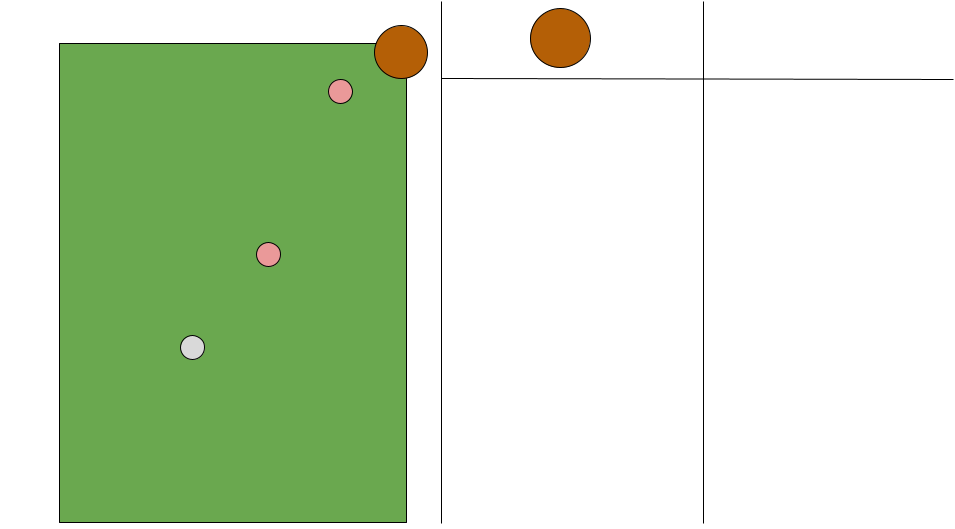
\includegraphics[width=0.5\linewidth]{../common/03_billiard_ai/resources/11_backwardsearch_1.png}
    \end{center}
    \caption{Kandidatensuche 1}
    \label{fig:backwardsearch_1}
\end{figure}

In einem zweiten Schritt wird die einzulochende Kugel definiert. Es kommen lediglich die beiden roten Kugeln in Frage.
Nachfolgend wird der Pfad weiter betrachtet, bei dem die rote Kugel, welche näher beim Loch ist, gewählt wurde.
Abbildung \ref{fig:backwardsearch_2} zeigt, dass der Suchbaum um einen Knoten erweitert wurde.
\begin{figure}[h!]
    \begin{center}
        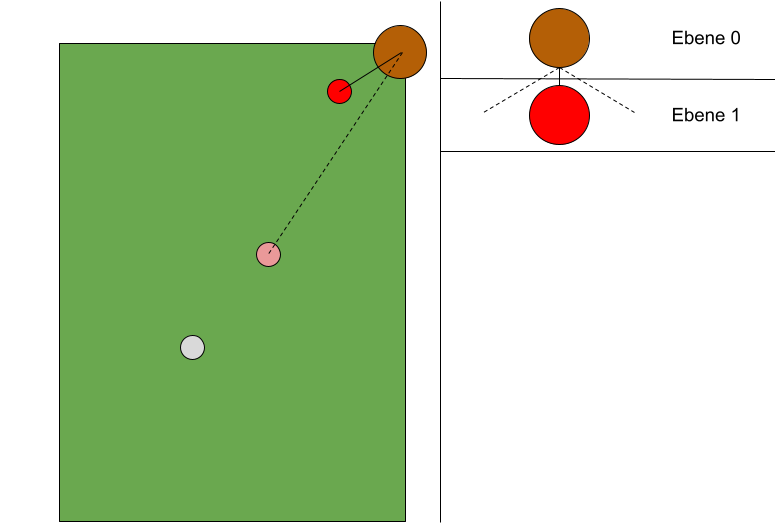
\includegraphics[width=0.5\linewidth]{../common/03_billiard_ai/resources/12_backwardsearch_2.png}
    \end{center}
    \caption{Kandidatensuche 2}
    \label{fig:backwardsearch_2}
\end{figure}

In Abbildung \ref{fig:backwardsearch_3} erfolgt der letzte Schritt. Hier sind verschiedene Optionen möglich, bspw.
könnte die weisse Kugel direkt oder über die Bande an die zuvor gewählte rote Kugel gespielt werden. Es könnte aber auch
die andere rote Kugel an die zuvor gewählte rote Kugel gespielt werden. Hier wird der Fall betrachtet, dass die weisse Kugel
indirekt über eine Bande an die zuvor gewählte rote Kugel gespielt wird.
\begin{figure}[h!]
    \begin{center}
        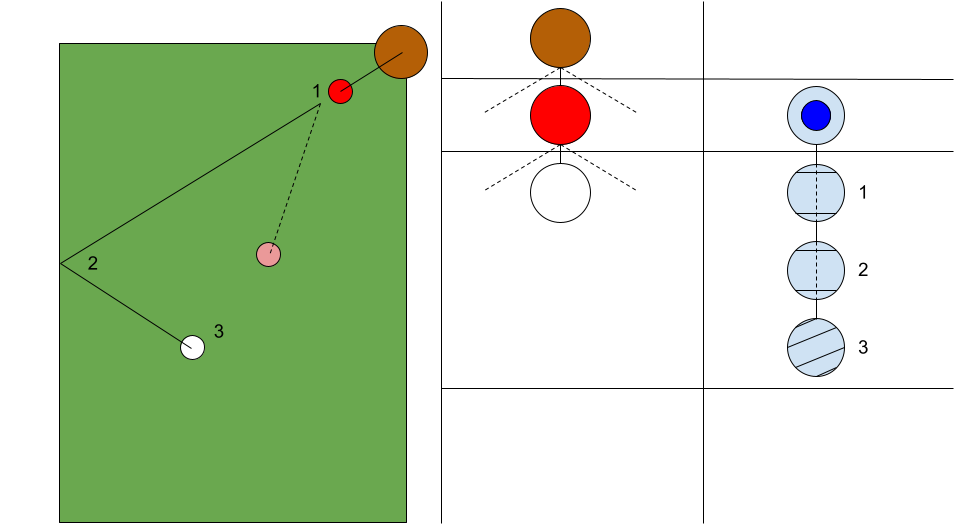
\includegraphics[width=0.5\linewidth]{../common/03_billiard_ai/resources/13_backwardsearch_3.png}
    \end{center}
    \caption{Kandidatensuche 3}
    \label{fig:backwardsearch_3}
\end{figure}

Algorithmus \ref{alg:backward_search} verdeutlicht den ablauf der \glqq Expand-Funktion\grqq. Zuerst wird eine
leere Liste namens \glqq nodes\grqq{} angelegt. Diese wird danach mit Nodes gefüllt, welche entweder durch einen Stoss
über eine weitere Kugel oder indirekt über die Bande zustande kommen. Die Nodes bilden das Ergebnis der Funktion.

\begin{algorithm}[H]
    \DontPrintSemicolon
    \SetKwFunction{expand}{expand}
    \SetKwProg{Fn}{Function}{}{}
    \Fn{\expand{node: Node, constantObjects: list} $\longrightarrow$ list[Node]}{
        nodes $\longleftarrow$ list()\\
        nodes $\longleftarrow$ append(expandBalls(node, constantObjects), nodes)\\
        nodes $\longleftarrow$ append(expandBank(node, constantObjects), nodes)\\
        \KwRet nodes
    }
    \caption{Algorithmus zur Durchführung eines Expansionsschritts bei der Kandidatensuche}
    \label{alg:backward_search}
\end{algorithm}
